\section{Extraction of Metals}

\begin{multicols}{2}


\section*{Chemical Properties of Metals}


\subsection{Ductility}

\begin{center}
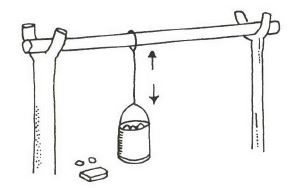
\includegraphics[width=0.4\textwidth]{./img/vso/ductility.jpg}
\end{center}

\begin{description*}
%\item[Subtopic:]{}
\item[Materials:]{Supports, metal wire, weights}
%\item[Setup:]{}
\item[Procedure:]{Suspend the wire between
supports and hang a weight onto
the free end. One method is
illustrated. Measure the length of
the wire. Add weights and the
wire will stretch.}
%\item[Hazards:]{}
%\item[Questions:]{}
%\item[Observations:]{}
\item[Theory:]{The physical strength, or \emph{tensile strength} of a metal is its ability to withstand applied force without breaking.}
%\item[Applications:]{}
\item[Notes:]{As an extension, compare the
ductility of wires made from
different metals.}
\end{description*}

\subsection{Malleability}

\begin{center}
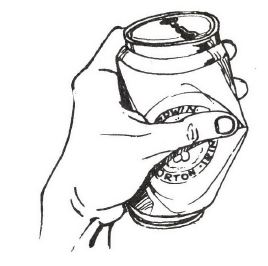
\includegraphics[width=0.35\textwidth]{./img/source/malleability.jpg}
\end{center}

\begin{description*}
%\item[Subtopic:]{}
\item[Materials:]{Aluminum can/roofing, hammer}
%\item[Setup:]{}
\item[Procedure:]{Hammer a crushed can, sheet of aluminium
roofing, a zinc case of a dry cell or any available
metal.}
%\item[Hazards:]{}
%\item[Questions:]{}
\item[Observations:]{The metal spreads out.}
\item[Theory:]{When force is applied the metal ions in the
giant metallic structure can move over each
other like ball bearings and hence spread out.}
%\item[Applications:]{}
%\item[Notes:]{}
\end{description*}

\columnbreak

\subsection{Conductivity}

\begin{center}
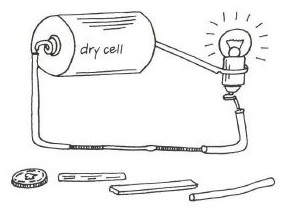
\includegraphics[width=0.4\textwidth]{./img/vso/conductivity.jpg}
\end{center}

\begin{description*}
%\item[Subtopic:]{}
\item[Materials:]{Dry cell, wires, bulb, metals (e.g. nail, zinc plate, copper wire, etc.), various items (e.g. graphite, pen, pencil, etc.)}
%\item[Setup:]{}
\item[Procedure:]{Set up the circuit as shown. Try various metals and non-metals to see which ones complete the circuit and light the bulb.}
%\item[Hazards:]{}
%\item[Questions:]{}
\item[Observations:]{Metals light the bulb.}
\item[Theory:]{Metals contain a "sea of electrons" which are
mobile. When these are made to flow in a
conductor with the aid of a battery an electrical
current flows and the bulb is lit. Non-metal
structures do not in general have this sea of
electrons except carbon in the form of graphite,
which has delocalised, mobile electrons between
the layers of carbon atoms.}
%\item[Applications:]{}
%\item[Notes:]{}
\end{description*}

%%% Moved to Ionic Theory and Electrolysis, Form III

%\subsection{Displacement of Copper} % Possible also in Ionic Theory and Electrolysis, Form III
%
%%\begin{center}
%%\includegraphics[width=0.4\textwidth]{./img/.jpg}
%%\end{center}
%
%\begin{description*}
%%\item[Subtopic:]{}
%\item[Materials:]{Steel wool, copper (II) sulphate, water, bottle}
%\item[Setup:]{Prepare a copper (II) sulphate solution by dissolving a spoonful of crystals in about 500 mL of water.}
%\item[Procedure:]{Pour 50 mL of the copper (II) sulphate solution into the container. Dip the steel wool into the solution and observe what happens.}
%%\item[Hazards:]{}
%%\item[Questions:]{}
%\item[Observations:]{A layer of brown copper metal forms on the surface of the steel wool (this is not rust).}
%\item[Theory:]{
%%This is an example of a displacement reaction - metal ions in the solution will reduce and metal solids will oxidize if the proper combination is used. Oxidized compounds lose electrons, while reduced compounds gain electrons. The iron metal oxidizes to form iron (II) ions and the copper (II) ions reduce to form copper metal.
%
%Metals can be arranged according to their reactivity, i.e. how likely they are to form positive ions. A metal higher in the reactivity series will displace a lower metal from a solution. 
%\begin{center}
%K $>$ Na $>$ Ca $>$ Mg $>$ Zn $>$ Fe $>$ Pb $>$ Sn $>$ H $>$ Cu $>$ Ag $>$ Au
%\end{center}
%Iron is higher than copper on the reactivity series, meaning iron ions displace copper ions in solution and the copper ions are deposited as copper metal. $$ \mathrm{CuSO}_{4(aq)} + \mathrm{Fe}_{(s)} \longrightarrow \mathrm{FeSO}_{4(aq)} + \mathrm{Cu(s)} $$}
%%\item[Applications:]{}
%%\item[Notes:]{}
%\end{description*}
%
%%\subsection{Displacement Reaction - Metal Reactivity} % Same as Displacement of Copper
%%
%%%\begin{center}
%%%\includegraphics[width=0.4\textwidth]{./img/.jpg}
%%%\end{center}
%%
%%\begin{description*}
%%%\item[Subtopic:]{}
%%\item[Materials:]{Nail, bottle, copper (II) sulphate}
%%%\item[Setup:]{}
%%\item[Procedure:]{Place the nail at the bottom of a container and cover it with copper (II) sulphate.}
%%%\item[Hazards:]{}
%%%\item[Questions:]{}
%%\item[Observations:]{In 5 minutes a reddish brown precipitate of copper will form.}
%%\item[Theory:]{This is an example of a displacement reaction - metal ions in the solution will reduce and metal solids will oxidize if the proper combination is used. Oxidized compounds lose electrons, while reduced compounds gain electrons. The iron metal oxidizes to form iron (II) ions and the copper (II) ions reduce to form copper metal, precipitating on the nail (this is not rust).}
%%%\item[Applications:]{}
%%\item[Notes:]{Repeat the activity using magnesium sulphate in place copper (II) sulphate. There will be no precipitate this time because the combination of compounds does not yield displacement.}
%%\end{description*}
%
%\subsection{Reactivity Series of Metals}
%
%\begin{center}
%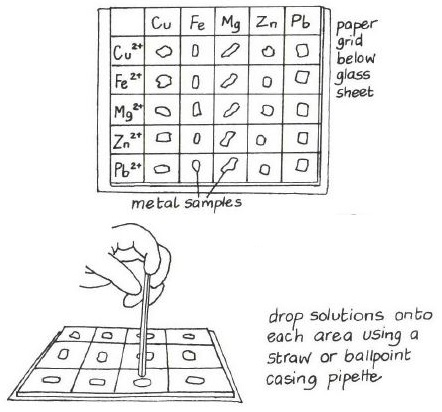
\includegraphics[width=0.49\textwidth]{./img/vso/reactivity-series.jpg}
%\end{center}
%
%\begin{description*}
%%\item[Subtopic:]{}
%\item[Materials:]{Glass sheet, large sheet of paper, metals, solutions of metal ions (see below)}
%\item[Setup:]{Gather and clean small pieces of various metals (e.g.copper wire, iron wool, magnesium ribbon, zinc plate from dry cell, lead shot). Gather some solutions containing metal ions (e.g. copper (II) sulphate, iron (II) sulphate, magnesium sulphate, zinc sulphate, lead nitrate).}
%\item[Procedure:]{Make a grid on the paper as shown. Place the glass sheet over the paper grid. Place the metals on the appropriate squares. Add 2-3 drops of a solution to each metal and observe and change.}
%%\item[Hazards:]{}
%%\item[Questions:]{}
%\item[Observations:]{On some of the squares a black or red (in the
%case of copper displacement) coating is formed
%on the surface of the metal.}
%\item[Theory:]{If a black coating forms on the metal it indicates that the metal ions are being displaced from the solution and deposited onto the metal. This shows that the metal is more reactive than the ion in solution. For example if Fe$^{2+}$ ions in
%solution are dropped onto magnesium, the
%magnesium displaces the Fe$^{2+}$ ions and a black
%coating of iron can be seen on the surface of the
%magnesium.}
%%\item[Applications:]{}
%%\item[Notes:]{}
%\end{description*}
%
%\subsection{Reactivity Rates Analogies}
%
%\begin{center}
%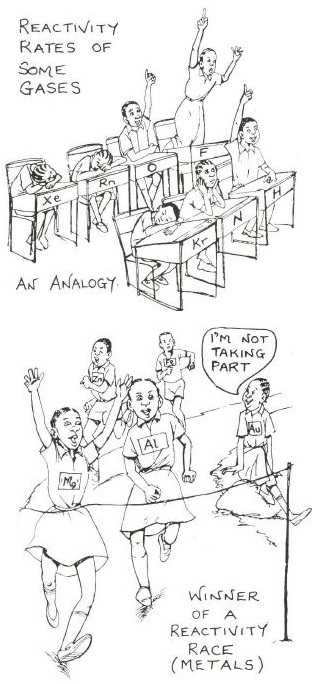
\includegraphics[width=0.4\textwidth]{./img/source/reactivity-rates-cartoons.jpg}
%\end{center}
%
%%\begin{description*}
%%%\item[Subtopic:]{}
%%\item[Materials:]{}
%%\item[Setup:]{}
%%\item[Procedure:]{}
%%\item[Hazards:]{}
%%\item[Questions:]{}
%%\item[Observations:]{}
%%\item[Theory:]{}
%%\item[Applications:]{}
%%\item[Notes:]{}
%%\end{description*}

%==================================================================================================%


\end{multicols}

\pagebreak